\chapter{Approach}
\label{chap:approach}
This chapter describes our approach to determine the mutation score of a source code unit under test based on source code and test suite metrics. In Section~\ref{sec:approach_tools} we first describe the tools and technologies used in our approach. Section~\ref{sec:approach_process} details the complete process for collecting our initial data. Then in Section~\ref{sec:approach_training}~\&~\ref{sec:approach_prediction} we describe how we use a SVM for training and prediction.


\section{Tools}
\label{sec:approach_tools}
The following sections show the tools selected for the technologies we are using in our approach. We selected our tools based on the ability to easily synthesis data to-and-from the tools. In addition, we preferred tools that give access to a \gls{cli}.


\subsection{Javalanche}
\label{subsec:approach_javalanche}
In our research we use Javalanche (version 0.4), a mutation testing tool for Java~\cite{SZ09} that applies a subset of the method-level mutation operators. Javalanche uses a subset of the method-level mutation operators (see Table~\ref{tab:javalanche_operators}). These selected operators provide a close approximation of the effectiveness of using the entire set of method-level operators at a reduced cost~\cite{OLR+96}.

\begin{table}[h]
  \centering
  \rowcolors{2}{gray!30}{gray!20}
  \begin{tabular}{|l|l|}
    \hline
    \rowcolor[RGB]{169,196,223}
    \textbf{Name} & \textbf{Description} \\
    \hline REPLACE\_CONSTANT & Replace a constant \\
    \hline NEGATE\_JUMP & Negate jump condition \\
    \hline ARITHMETIC\_REPLACE & Replace arithmetic operator \\
    \hline REMOVE\_CALL & Remove method call \\
    \hline REPLACE\_VARIABLE & Replace variable reference\\
    \hline ABSOLUTE\_VALUE & Insert absolute value of a variable \\
    \hline UNARY\_OPERATOR & Insert unary operator \\
    \hline
  \end{tabular}
  \caption{The set of selective method-level mutation operators used in Javalanche.}
  \label{tab:javalanche_operators}
\end{table}

We chose Javalanche for our research because it is customizable and extensible, therefore allowing us to modify Javalanche to calculate unit mutation scores and output a richer set of results. Other benefits of Javalanche include (see Table~\ref{tab:mutation_tools} for all features): full integration with JUnit, the use of mutation schemas and bytecode generation to improve performance and, test selection using coverage. Although Javalanche does not have class-level mutation operators, due to the open source nature of Javalanche we plan to extend it to incorporate class-level mutation operators. In addition, Javalanche does have concurrency-level mutation operators as well as the ability to identify equivalent mutants using impact analysis.


\subsection{LIBSVM}
\label{subsec:approach_libsvm}
In our research we use LIBSVM (version 3.12), a \gls{svm} library capable of solving \emph{n}-group classification problems~\cite{CL11}. We decided to use this library implementation as it is mature and used in many other publications\footnote{LIBSVM~\cite{CL11} has been cited 9323 times according to Google Scholar as of May 21$^{st}$, 2012}. LIBSVM has the ability to run entirely from a \gls{cli}, and provides an easy to use interface to perform training and prediction.


\subsection{Eclipse Metrics Plugin}
\label{subsec:approach_metrics_plugin}
In our research, we use the Eclipse Metrics Plugin (version 1.3.8.20100730-001) to acquire source code metrics of the method- and class-level source code unit under test~\cite{Metrics}. We selected this tool as it provides a comprehensive set of metrics for Java programs (see feature sets \ding{172}~\&~\ding{174} from Table~\ref{tab:metrics}). The metrics can also be exported to \gls{xml} which is a suitable format to extract data from. Though this tool is part of Eclipse as a plugin it is possible to initiate the tool through a \gls{cli} interface after importing the \gls{sut} into Eclipse.


\subsection{EMMA}
\label{subsec:approach_emma}
We focus on JUnit test cases as our testing framework, thus can actually use the Eclipse Metrics Plugin to gather the source code metrics of the test suite (see feature set \ding{175} from Table~\ref{tab:metrics}). In order to gather other test suite coverage metrics we use EMMA (version 2.0.5312) which is capable of determining the basic block coverage of a test suite~\cite{EMMA}. Specifically, we use EMMA to acquire metrics for feature set \ding{173} from Table~\ref{tab:metrics}.


\section{Process}
\label{sec:approach_process}
Our process for mutation score prediction using source code and test suite metrics is shown in Figure~\ref{fig:process}. As we are using a supervised learning technique for prediction, a \gls{svm}, we need to initially collect training data. Thus we inevitably have to calculate the mutation scores of a software system at least once. As mentioned in the motivation (see Section~\ref{sec:introduction_motivation}) our approach aims to reduce the amount of mutation testing done in iterative development. If our technique generalize well then it can be possible to build a comprehensive model and predict on different software systems without any prior mutation testing (we explore this in Chapter~\ref{??}). The following sections walk through the complete process one phase at a time, providing examples where possible.

\begin{figure}[h]
  \centering
  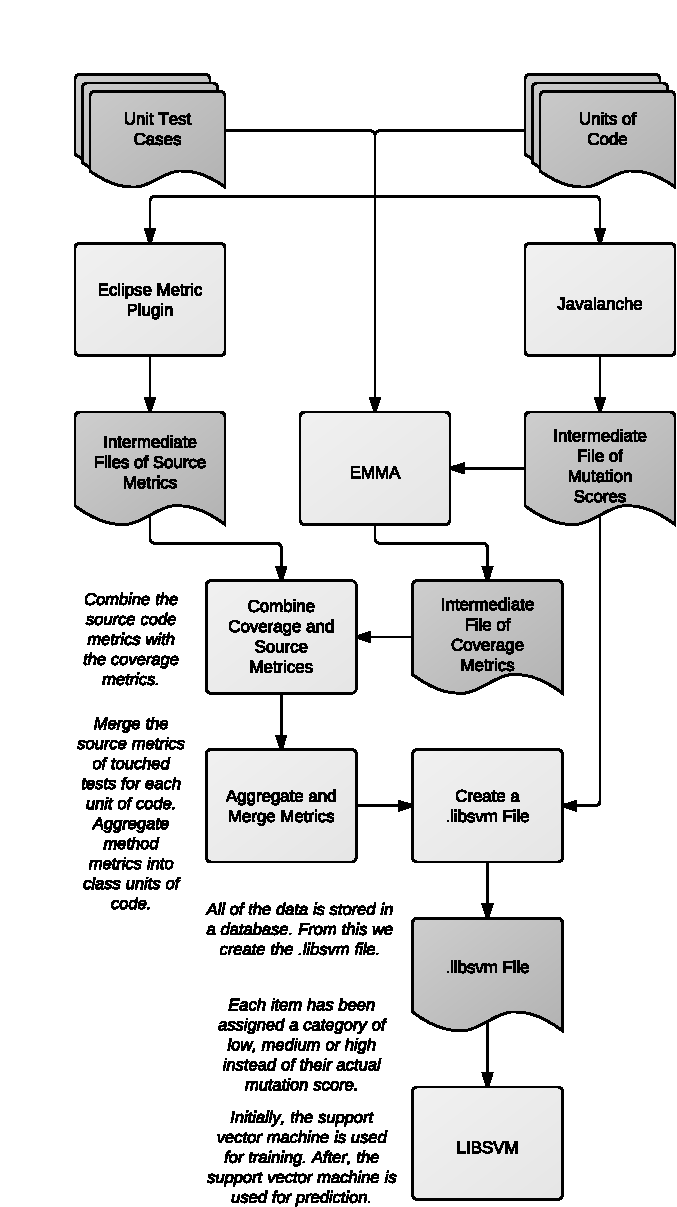
\includegraphics[width=11cm]{figures/process.pdf}
  \caption{The complete process for collecting data used to training a SVM to predict mutation scores.}
  \label{fig:process}
\end{figure}


\subsection{Inputs}
\label{subsec:appraoch_inputs}
To predict the mutation score of source code units (methods and classes) our approach requires the following inputs: a set of source units of code (the Java files that compose the \gls{sut}) and the corresponding set of unit test cases (the JUnit files that compose the test suite for the \gls{sut}). A simple example of the input our approach requires is presented in Figure~\ref{fig:triangle_example}. Our approach is only concerned with source units of code that are being tested, thus the more coverage the test suite provides the more data that can be extracted from the \gls{sut}.

\begin{figure}[h]
  \centering
  \begin{minipage}{6.75cm}
  \centering
  \footnotesize{\textbf{\texttt{Triangle} Source Code}}
  \lstinputlisting[language=Java]{listings/Triangle.java}
  \end{minipage}
  \qquad
  \begin{minipage}{6.75cm}
  \centering
  \footnotesize{\textbf{\texttt{TriangleTest} Test Suite}}
  \lstinputlisting[language=Java]{listings/TriangleTest.java}
  \end{minipage}
  \caption{Example source code of \texttt{Triangle} and its test suite \texttt{TriangleTest}.}
  \vspace{1mm}
  \footnotesize{Figure~\ref{fig:triangle_example} presents a stripped down example of expected input that our prediction approach requires. This system has a single method to classify triangles, along with a few test cases to test its capabilities in classifying triangles.}
  \vspace{1mm}
  \label{fig:triangle_example}
\end{figure}


\subsection{Collect Source Code Metrics}
\label{subsec:appraoch_collect_source_metrics}
Given our input of the software system we first must acquire the source code metrics of the source code units and the unit test cases. We use the Eclipse Metrics Plugin to analyze the software system to produce an \gls{xml} file of the source code metrics. The produced \gls{xml} file is \emph{metric-oriented}, so we translate so it is \emph{unit-oriented}. This phase acquires the source code metrics (see feature set \ding{172}) for each source code unit and unit test case. Using the example in Figure~\ref{fig:triangle_example} this phase extracts the following metrics as seen in Table~\ref{tab:triangle_class_extracted_metrics}~\&~\ref{tab:triangle_method_extracted_metrics}.

\begin{landscape}
  \begin{table}[h]
    \centering
    \rowcolors{2}{gray!30}{gray!20}
    \begin{tabular}{|l|r|r|}
      \hline
      \rowcolor[RGB]{169,196,223}
      \textbf{Metrics} & \texttt{\textbf{Triangle}} & \texttt{\textbf{TriangleTest}} \\
      \hline NORM & 0 & 0 \\
      \hline NOF & 0 & 0 \\
      \hline NSC & 0 & 0 \\
      \hline DIT & 1 & 1 \\
      \hline LCOM & 0 & 0 \\
      \hline NSM & 1 & 0 \\
      \hline NOM & 0 & 5 \\
      \hline SIX & 0 & 0 \\
      \hline WMC & 18 & 5 \\
      \hline NSF & 0 & 0 \\
      \hline
    \end{tabular}
    \caption{Extracted class source code metrics of the \texttt{Triangle} system.}
    \label{tab:triangle_class_extracted_metrics}
  \end{table}

  \begin{table}[h]
    \centering
    \rowcolors{2}{gray!30}{gray!20}
    \begin{tabular}{|l|r|r|r|r|r|r|}
      \hline
      \rowcolor[RGB]{169,196,223}
      \textbf{Metrics} & \texttt{\textbf{classify}} & \texttt{\textbf{testScalene}} & \texttt{\textbf{testIsoceles}} & \texttt{\textbf{testEquiliteral}} & \texttt{\textbf{testNegative}} & \texttt{\textbf{testInvalid}} \\
      \hline MLOC & 24 & 2 & 2 & 2 & 2 & 2 \\
      \hline NBD & 1 & 1 & 1 & 1 & 1 & 1 \\
      \hline VG & 18 & 1 & 1 & 1 & 1 & 1 \\
      \hline PAR & 3 & 0 & 0 & 0 & 0 & 0 \\
      \hline
    \end{tabular}
    \caption{Extracted method source code metrics of the \texttt{Triangle} system.}
    \label{tab:triangle_class_extracted_metrics}
  \end{table}
\end{landscape}


\subsection{Collect Test Suite Coverage Metrics}
\label{subsec:appraoch_collect_coverage_metrics}


\subsection{Combine Coverage and Source Metrics}
\label{subsec:appraoch_combine_metrics}


\subsection{Aggregate and Merge Method-Level Metrics}
\label{subsec:appraoch_aggregate_merge_metrics}
\begin{table}[h]
  \centering
  \rowcolors{2}{gray!30}{gray!20}
  \begin{tabular}{|l|l|l|l|}
    \hline
    \rowcolor[RGB]{169,196,223}
    \textbf{Metrics} & \textbf{Description} & \textbf{Scope} & \textbf{Set} \\

    % Set 1: Source Code Metrics
    \hline MLOC & Method lines of code & Method & \ding{172} \\
    \hline NBD & Nested block depth & Method & \ding{172} \\
    \hline VG & McCabe cyclomatic complexity & Method & \ding{172} \\
    \hline PAR & Number of parameters & Method & \ding{172} \\
    \hline NORM & Number of overridden methods & Class & \ding{172} \\
    \hline NOF & Number of attributes & Class & \ding{172} \\
    \hline NSC & Number of children & Class & \ding{172} \\
    \hline DIT & Depth of inheritance tree & Class & \ding{172} \\
    \hline LCOM & Lack of cohesion of methods & Class & \ding{172} \\
    \hline NSM & Number of static methods & Class & \ding{172} \\
    \hline NOM & Number of methods & Class & \ding{172} \\
    \hline SIX & Specialization index & Class & \ding{172} \\
    \hline WMC & Weighted method per class & Class & \ding{172} \\
    \hline NSF & Number of static attributes & Class & \ding{172} \\

    % Set 2: Coverage Metrics
    \hline BCOV & Basic blocks covered in code unit & Class/Method & \ding{173} \\
    \hline BTOT & Total basic blocks for code unit & Class/Method & \ding{173} \\
    \hline NOT & Number of test cases & Class/Method & \ding{173} \\

    % Set 3: Accumulated Source Code Metrics
    \hline SMLOC & Sum MLOC of methods & Class & \ding{174} \\
    \hline SNBD & Sum NBD of methods & Class & \ding{174} \\
    \hline SVG & Sum VG of methods & Class & \ding{174} \\
    \hline SPAR & Sum PAR of methods & Class & \ding{174} \\
    \hline AMLOC & Average MLOC of methods & Class & \ding{174} \\
    \hline ANBD & Average NBD of methods & Class & \ding{174} \\
    \hline AVG & Average VG of methods & Class & \ding{174} \\
    \hline APAR & Average PAR of methods & Class & \ding{174} \\

    % Set 4: Accumulated Test Case Metrics
    \hline STMLOC & Sum MLOC of test methods & Class/Method & \ding{175} \\
    \hline STNBD & Sum NBD of test methods & Class/Method & \ding{175} \\
    \hline STVG & Sum VG of test methods & Class/Method & \ding{175} \\
    \hline STPAR & Sum PAR of test methods & Class/Method & \ding{175} \\
    \hline ATMLOC & Average MLOC of test methods & Class/Method & \ding{175} \\
    \hline ATNBD & Average NBD of test methods & Class/Method & \ding{175} \\
    \hline ATVG & Average VG of test methods & Class/Method & \ding{175} \\
    \hline ATPAR & Average PAR of test methods & Class/Method & \ding{175} \\
    \hline
  \end{tabular}
  \caption{The complete set of metrics used as attributes for each vector of the \gls{svm}.}
  \vspace{1mm}
  \footnotesize{\emph{Table~\ref{tab:metrics} shows the complete set of metrics used as attributes for each vector of the \gls{svm}, categorized by feature set (\ding{172}: Source Code Metrics, \ding{173}: Coverage Metrics, \ding{174}: Accumulated Source Code Metrics, \ding{175}: Accumulated Test Case Metrics).}}
  \vspace{1mm}
  \label{tab:metrics}
\end{table}


\subsection{Collect Mutation Scores}
\label{subsec:appraoch_collect_mutation_scores}


\subsection{Create LIBSVM File}
\label{subsec:appraoch_create_libsvm_file}


\section{Training}
\label{sec:approach_training}
Our training process requires as input a set of units of code and for each code unit a corresponding set of unit test cases. Both the code units under test and test cases (i.e., JUnit tests) are Java source files.

The first step of our process is to collect the two types of data required to train the SVM:

\begin{itemize}
  \item \textbf{Category Data:} Javalanche is used to generate the mutants of all code units in the project under test and to perform the mutation testing by executing the required tests for each mutant. It should be noted that currently our Javalanche configuration does not exclude equivalent mutants from the analysis. For our research, we added a new analyzer component to Javalanche that outputs an intermediate text file of mutation scores of the covered units (methods and classes).

  \item \textbf{Feature Data:} The feature data is comprised of the source code and test suite metrics (see Table~\ref{tab:metrics} for feature sets referenced in the following text). By using the Eclipse Metric Plugin we collect source code metrics (sets \ding{172}~\&~\ding{174}) for both method- and class-level code units. We also collect the test suite metrics (set \ding{175}) of each unit's test cases using the Eclipse Metric Plugin. Test suite coverage metrics (set \ding{173}) are obtained using the EMMA tool.
\end{itemize}

Next, we create a .libsvm file containing the category and feature data from the database. Instead of predicting a specific mutation score percentage, we categorize all mutation scores as \textit{low, medium, high} which reduces the mutation score prediction to a three-group classification problem. The ranges of values in each category are determined based on the distribution of the mutation scores in our training data (further explained in Section~\ref{sec:experiment_results}). Finally, the .libsvm file is passed into LIBSVM to complete the training process.


\section{Prediction}
\label{sec:approach_prediction}
Once we have trained the SVM, we can then use the SVM for prediction. We can predict the mutation score category of an unknown unit of code by first determining the source code and test suite metrics. The metrics (i.e., features) are passed into the SVM which will then assign a category of \textit{low, medium, high} for the mutation score.  Currently, our approach only predicts mutation scores within a project. That is, the training and prediction data both come from the same project repository.


\section{Related Work}
\label{sec:approach_related_work}
The use of software metrics to locate faults in source code has been well researched. For example, Koru et al. utilized static software measure along with defect data at the class level to predict bugs using machine learning~\cite{KL05}. Similarly, Gyimothy et al. used object-oriented metrics with logistic regression and machine learning techniques to identify faulty classes in open source software~\cite{GFS05}. Finally, design level metrics were used with a linear prediction model to determine the estimated maintainability and error prone modules of large software systems~\cite{MKPS00}. Our work is unique in comparison to these previous works since we not only use source code metrics but we also use test suite metrics to enhance our predication capabilities.
